\begin{homeworkProblem}[Quiz 2, Problem 2] 
    Okay, the problem of solving for the z-component of the electric
    field generated by a charged disk seemed to be difficult for you
    guys. Let me discuss a few ways in which this problem could be
    solved.
    
    The first approach that I will use will be to establish the
    electric field set up by a ring centered around the z-axis. Then, I
    will integrate over an infinite number of rings whose radius varies
    smoothly from 0 to the radius of the disk.

    The second approach that I will use will be to establish the
    electric field from a disk directly using polar coordinates. I will
    integrate around the disk (in the angular direction) and I will
    integrate radially outward (from 0 to R, the radius of the disk).
    This involves the use of the differential area alement $\diff a$ in
    polar coordinates. I will try my best to explain the origins of this
    differential area element. That may go in an appendix at the end.

    \begin{homeworkSection}{Approach 1}
        Okay, so I'm going to first start by solving for the electric
        field established by a uniformly charged ring. The ring will
        have a constant charge per unit length, $\lambda$, such that the
        total charge on the ring is $2\pi R \lambda = Q$. My approach
        will be to chop up the ring into a bunch of infinitesimal point
        charges $\diff q'$ and evaluate the electric field, $\diff \vec{E}$,
        generated by each of these infinitesimal point charges. Once I
        have this contribution to the electric field I will integrate
        over all the infinitesimal point charges to find the net
        electric field $\vec{E} = \int \diff \vec{E}$. 

        \begin{figure}[t]
            \centering    
            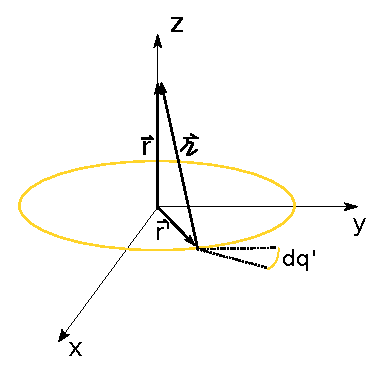
\includegraphics{./img/ringofcharge.eps}
            \caption{Ring of charge centered along z-axis}
            \label{fig:roc.eps}
        \end{figure}

        The key to starting to write this integral is to realize that
        each infinitesimal check of charge $\diff q'$ is like a little point
        charge located at position $r'$ (see figure \ref{fig:roc.eps})
        and, as such, the electric field contribution due a particular
        chunk of charge, $\diff q'$, looks like:

        \[ \diff \vec{E}(\vec{r}) = \frac{k \diff q'}{|\vec{\scriptr}|^2}
        \hat{\scriptr} \]

        Now, $\diff q'$ really describes the position of a chunk of charge
        $\diff q'$ located at $\vec{r'}$. The infinitesimal chunk of charge
        can be written as $\diff q' = \lambda \diff l'$, where $\diff
        l'$ is an infinitesimal arc length along the path of the ring.

        Thus, my expression for $\diff \vec{E}(\vec{r})$ looks like
        
        \[ \diff \vec{E}(\vec{r}) = \frac{k \lambda \diff l'}{|\vec{\scriptr}|^2}
        \hat{\scriptr} \]

        But, $\diff l'$ just represents a little arc length. We know
        that an arc length $s$ can be related to the radius of the
        circle and the swept (subtended) angle, $\theta$ can be written
        as $s = R \theta$. Thus, I will write the arc length $\diff l'$
        as $\diff l' = R \diff \theta'$ so that $\diff \vec{E}(\vec{r})$
        becomes:


        \[ \diff \vec{E}(\vec{r}) = \frac{k \lambda R \diff
        \theta'}{|\vec{\scriptr}|^2} \hat{\scriptr} \]

        Now, our expression is looking more and more like something we
        can integrate. However, we should really right $\vec{\scriptr}$
        in terms of something we know. What is $\vec{\scriptr}$?
        Remember, this vector points from the point where the charge
        that we're considering is located to the point where we would
        like to evaluate the electric field. Thus, in terms of
        $\vec{r}$, the vector that points from the origin to where we
        would like to evaluate the electric field and $\vec{r'}$, the
        vector that points from the origin to the chunk of charge we're
        considering $\vec{\scriptr} = \vec{r}-\vec{r'}$. In order to put
        this into my expression for $\diff \vec{E}$ I need to scale
        thetope and bottom by the magnitude of $\vec{\scriptr}$ to get
        rid of that pesky unit vector. Doing this yields:
        
        \[ \diff \vec{E}(\vec{r}) = \frac{k \lambda R \diff
        \theta'}{|\vec{\scriptr}|^3} \vec{\scriptr} \]

        Performing my substitution for $\vec{\scriptr}$ yields:

        \[ \diff \vec{E}(\vec{r}) = \frac{k \lambda R \diff
        \theta'}{|\vec{r}-\vec{r'}|^3} (\vec{r} - \vec{r'}) \]

        Now, can we simplify this expression at all before we integrate?
        Yes! We know that $\vec{r} = z \hat{z}$ since we are only
        solving for the electric field along the z-axis. We also know
        that $|\vec{\scriptr}|$ is $\sqrt{R^2+z^2}$ (look at
        \ref{fig:roc.eps})
        Performing these substitutions yields:

        \[ \diff \vec{E}(z) = \frac{k \lambda R \diff
        \theta'}{(R^2+z^2)^{1.5}} (z \hat{z}- \vec{r'}) \]

        Now, we can almost perform this integral. We just need an
        expression for $\vec{r'}$ in terms of $\theta'$ so that we can
        perform the integral over $\theta'$. But, $\vec{r'} =
        R\cos(\theta')\hat{x} - R\cos(\theta')\hat{y}$. This can be seen
        by considering how $\vec{r'}$ must change direction as a
        function of $\theta'$. Now, we just plug this into our previous
        expression and integrate over $\theta'$ from $0 \rightarrow
        \pi/2$.

        \[ \vec{E}(z) = \int\limits_0^{2\pi} k \lambda R \frac{ \diff
        \theta'}{(R^2+z^2)^{1.5}} (z \hat{z}-
        R\cos(\theta')\hat{x}+R\cos(\theta')\hat{y}) \]

        Now, k and $\lambda$ are constants that I can pull out of the
        integral. The integrals over $\cos\theta'$ and $\sin\theta'$ I
        already know are going to go away. I know this because
        $\int_0^{2\pi} \cos\theta \diff \theta = \int_0^{2\pi}
        \sin\theta \diff \theta = 0 $. Thus, only the $\hat{z}$
        component survives the integral (like we'd expect) and the
        integral reduces to:

        \[ \vec{E}(z) = \int\limits_0^{2\pi} k \lambda R \frac{ \diff
        \theta'}{(R^2+z^2)^{1.5}} z \hat{z} \]

        Notice that everything inside the integral is a constant with
        respect to $\theta'$ except for our integration differential
        $\diff \theta'$. Thus, the integral is just:

        \[ \vec{E}(z) = \frac{k\lambda R 2\pi z
        \hat{z}}{(R^2+z^2)^{1.5}} \]

        This looks a little ugly. Once we realize that $2\pi R \lambda$
        is just $Q$, thet total charge on the ring (the charge per unit
        length on the ring times the total length of the ring) we can
        simplify this to:

        \[ \vec{E}(z) = \frac{k Q }{(R^2+z^2)^{1.5}} z\hat{z} \]

        Note that this expression depends on the radius of the ring. Our
        next goal will be to integrate over a bunch of rings with
        different radii to obtain the electric field along the z-axis
        due to a charged disc. Thus, I'm going to chop the electric
        field for the disc up into a bunch of rings.
   
        \[ \diff \vec{E}(z) = \frac{k dQ}{(R^2+z^2)^{1.5}} z\hat{z} \]

        \begin{figure}[t]
            \begin{center}
                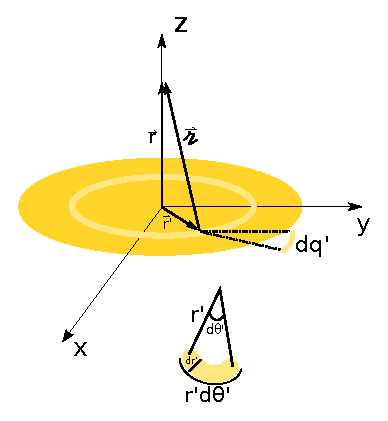
\includegraphics{./img/discofcharge.eps}
            \end{center}
            \caption{Disc of charge broken up into rings}
            \label{fig:doc.eps}
        \end{figure}

        What is dQ? Well, dQ is me treating each ring as a chunk of
        charge that generates a little portion of the total electric
        field. Now, since I'm integrating over rings to form a disc I
        need to give these rings some infinitesimal width. The disc will
        be formed of a bunch of rings of infinitesimal width. A ring of
        infinitesimal width and of radius $R'$ will have an amount of
        charge equal to $2 \pi R' dR' \sigma$ (see \ref{fig:doc.eps} and
        allow $\diff \theta'$ to be $2 \pi$ - you might argue that this
        is not an infinitesimal quantity\dots well it turns out that
        this doesn't matter. It's still the area of that ring: $2\pi r'
        dr'$). What is $\sigma$? It's the surface charge density. Since
        we're considering areas of charge, now, we need to consider area
        charge densities. Think about whether a relationship can be
        drawn between $\lambda$ and $\sigma$. Let's try to write down
        the integral now that we know what $\diff Q$ is.

        \[ \vec{E}(z) = \int_0^{R_{disc}} \diff \vec{E}(z) =
        \int_0^{R_{disc}}\frac{k 2 \pi R' dR' \sigma}{(R'^2+z^2)^{1.5}}
        z\hat{z} \]

        Now, this integral is not hard to solve. I'll pull out the
        constants so that the math is a little more transparent. 
        
        \[ \vec{E}(z) = \int_0^{R_{disc}} \diff \vec{E}(z) =
        2\pi \sigma z \hat{z} \int_0^{R_{disc}}\frac{R' dR'
        }{(R'^2+z^2)^{1.5}} \tag{1} \]
        
        Now, I solved this using WolframAlpha but this type of integral
        can be solved with a simple u-substitution (allow $u = R'^2 +
        z^2$ so that $\frac{\diff u}{\diff r} = 2 R' dR'$).

        The final result, after doing all of this is that:

        \[ \vec{E}(z) = k\sigma 2\pi \bigg( 1 - \frac{z}{z^2+R_{disc}^2}
        \bigg)\hat{z} \]

        %\[ \vec{E}_{disc}(z) = \int_0^{R_{disc}}\frac{k Q(R) \diff R
        %}{(R^2+z^2)^{1.5}} z\hat{z} \]

        %The reason that Q is now a function of R is that we want to
        %describe the electric field generated by a bunch of rings. In
        %order that the disc have a uniform charge density over its area,
        %each of the constituent rings need a uniform charge density over
        %their own circumferences. Thus, for a larger ring, there exists
        %more charge on that ring.

        %What is $Q(R)$? Well that's a good question. We know that $Q =
        %2\pi\lambda R$. This must be $Q(R)$. That makes sense. Let's
        %plug this in.
        
        \end{homeworkSection}
    
    \begin{homeworkSection}{Approach 2}

        Now, that was super tedious. Let's try this another way. Let's
        now break the disc up into a little bunch of patches of area
        $da$ instead of a bunch of rings of infinitesimal thickness. If
        we do this, we need to think about how best to think about the
        area of the disc.
        
        If we break the disc up into a bunch of
        rectangular areas, $da$, like is done with Cartesian coordinates
        we will have a difficult time integrating over our disc (see
        %\ref{fig:patches.eps}
        . Our bounds will have to be over the area of the disc which
        require that we express the limits of our integral in terms of
        the equation of the circle. I don't really want to deal with $y
        = \pm \sqrt{1-x^2}$ in my limits.


        Instead, let's consider the patches of area to be little arcs of
        some finite thickness. See \ref{fig:doc.eps} for a decent visual
        explanation.  Now, it's easy to break up the area of our circle
        into little chunks. We will talk about a little chunk of area
        $da = (R \diff \theta)(\diff R)$. That is, the little chunk will
        have an arclength that is $R \diff \theta$ long and $\diff R$
        wide. That determines the area of this patch. You can convince
        yourself, easily, that this is a great way to think about areas
        when it comes to dealing with problems with circles in them.
        Let's integrate the area of a circle with these coordinates:

        \begin{align}
            A &= \int_0^R da \nonumber \\
            &=  \int_0^R \int_0^{2\pi} r \diff r \diff \theta
            \nonumber \\
            &= \int_0^R r \diff r \int_0^{2\pi} \diff \theta \nonumber \\
            &= \frac{r^2}{2}\big|_0^R \quad \theta\big|_0^{2\pi}
            \nonumber \\
            &= \pi R^2 \nonumber 
        \end{align}

        So, although this isn't a proof, it should at least be
        convincing evidence that maybe this is a good expression to use
        for the differential area element when we're dealing with
        circles. Now, I'm going to immediately write the integral we're
        going to solve since the approach is very similar to what we'va
        already done.

        \[ \vec{E}(z) = \int_0^{2\pi} \int_0^R \frac{k dq' (z \hat{z}-
        r'\cos(\theta')\hat{x}+r'\cos(\theta')\hat{y})}{(z^2+r'^2)^{1.5}}
        \]

        Now, $r'$ describes the distance the infinitesimal chunk of
        charge is away from the origin. $\theta$ describes the location
        of that chunk with respect to the x-axis. Thus, by sweeping over
        all $\theta': 0 \rightarrow 2\pi$ and all $r': 0 \rightarrow R$ we
        sweep over all the charge. Now, we just have to right $dq'$ in
        terms of $r'$ and $\theta'$ and we're good. But, $dq' = \sigma
        \diff a' = \sigma r' dr' \diff \theta'$, from the earlier
        discusson. The integral now reads:

        \[ \vec{E}(z) = \int_0^{2\pi} \int_0^R \frac{k \sigma r' dr'
        \diff \theta' (z \hat{z}-
        r'\cos(\theta')\hat{x}+r'\cos(\theta')\hat{y})}{(z^2+r'^2)^{1.5}}
        \]

       Right away I'm going to realize that the integral over the
       $\hat{x}$ and the $\hat{y}$ components go away because I'm
       integrating $\sin\theta'$ and $\cos\theta'$ over one period (from
       0 to $2\pi$).

        \[ \vec{E}(z) = \int_0^{2\pi} \int_0^R \frac{k \sigma r' dr'
        \diff \theta' (z \hat{z} }{(z^2+r'^2)^{1.5}}
        \]

        Now, the only $\theta'$ in my integral is the $\diff \theta'$.
        So, I can evaluate the integral over $\diff \theta'$ very
        easily. 

        \[ \vec{E}(z) = 2\pi \int_0^R \frac{k \sigma r' dr'
        (z \hat{z} }{(z^2+r'^2)^{1.5}}
        \]

        I then realize that this is the same integral as the one I was
        doing earlier (see Equation 1). Thus, the result must be the
        same. This is an easier, less confusing way to get the electric
        field for a disc along the z-axis.

    \end{homeworkSection}    
\end{homeworkProblem}
